\chapter{Evaluation}
Given that design usability was the salient point of this project, a user study was a good way to assess its performance. After gaining approval from the Ethics board, a pilot study was run, followed by the actual user study. The results confirm the hypotheses - users learnt how to use the system after one use, and they were able to modify their chart faster in Sketchography compared to Excel. A description of the study and a summary of the results follows; for the entire questionnaire and full data analysis, see \autoref{cha:questionnaire} and \autoref{cha:analysis}.
%TODO Maybe add a qualitative example here of horribly drawn charts being correctly identified. Or atleast mention that the recognition works remarkably well.

\section{Study Goals}
In the Introduction (\autoref{cha:introduction}), I hypothesized that the direct manipulation and liveness of this system would offer two advantages:

\begin{enumerate}
\item[H1] This interface is more `learnable' over time
\item[H2] It encourages exploratory data visualisation creation by making modification easier
\item[H3] Its advantages hold independent of how fluent the user is in English.
\end{enumerate}

The study was designed to evaluate whether these three properties were achieved. 

\subsection*{Learnability}
To investigate whether the interface is learnable over time, users were asked to carry out a very similar task twice, and their times across tasks were compared. If the user shows a statistically significant improvement in the time taken to carry out the task, then they are learning how to use the interface, and becoming adept at using it. The chosen task is to import (mock) data and create a bar chart.

To make this experiment fair, the tasks had to be phrased very carefully. The tasks had to be very similar, to make sure one was not systematically harder or easier, but not so similar that users could mechanically follow the same steps without even understanding the problem.

In addition, the tasks had to tell the user what output is expected, without explicitly listing every single step required to get there. This did not hold true for the version of the task descriptions used in the pilot, an example of which is below.

\begin{quotation}
Task A:
\begin{enumerate}
\item Load the `Task A.xlsx' file.
\item Create a bar chart of `Births' and `Deaths', with `Year' on the X Axis.
\end{enumerate}
\end{quotation}

Clearly, this would leave little room for users to demonstrate that they have learnt how to use the application, since the task guides them through exactly what they need to do. Thus, the task was rephrased to focus on the problem (note, the data schema of the file was also changed to focus on differences between countries rather than years).

\begin{quotation}
Task A:

You work in a government agency and are trying to see how population is growing in 4 different countries. The ‘Task A’ file contains information regarding how many births and deaths occurred in 1 year in each country (the numbers are scaled to account for population). 

Use the Sketchography app to create a column bar chart that will allow someone to compare birth and death rates across the countries.

Speak out aloud the name of the country where the population is declining (where the death rate is larger than the birth rate).

\end{quotation}

This is better, since the user now needs to understand the context of the problem, grasp which data is relevant and which fields need to go on each axis for them to notice the trend required.

\subsection*{Modification}
To see whether the interface enables quick exploration, the time required to make a specific modification in Sketchography needed to be compared to the time required for the same modification in users' usual chart editor. The only other chart editor we compared was Microsoft Excel, which proved a sensible decision since all the final study participants indicated that Excel was their tool of choice for making charts, and only 2 out of 10 had actually used anything else to create a chart.

To make the comparison fair, we needed a modification that was a reasonable change to make quickly, and was supported by both editors. Two such changes are to change the width of the bars, and to change the height of the bars, without changing the dimensions of the chart itself. In the pilot study, some participants were asked to change the height, while others were asked to change the width. However, in Excel, the user has no direct control over the width of the bars. Instead, they have to do this indirectly by changing a 'Gap Width' setting, which controls the space between the bars. This indirection was not a perfect analogue to the method to change the bar width in Sketchography, so some users never identified how to make this change. Thus, in the final user study, we focused instead on changing just the height of the bar, which could be done via similar settings in both applications.

The users weren't shown how to make this change, or that the option was only available in the formal view (since stylus interaction with the chart in sketch view would be interpreted as ink). They had to explore the User Interface and discover the way to do this themselves. The method involved hovering over a bar in the data series, which exposes a drag handle on the top and the right of the bar. The top one can be dragged to manipulate the height (more specifically, the Y axis scale). In Excel, it involved opening an `Action Pane' by double clicking on a bar, or right clicking on it and then selecting the right option, or via a button in the ribbon interface on the top of the screen. In this `Action Pane', there was a setting to change the Y axis scale.

\subsection*{Language Independence}
A secondary benefit of the direct manipulation and visual metaphors is that Sketchography isn't as language dependent as a system with configuration dialogues in English. Users should be able to learn Sketchography just as quickly whether they speak English as their primary language or not. 

India is a nation of multiple languages, but a lot of businesses conduct their activities in English. By carrying out the study there, participants with varied levels of fluency in English can be recruited.

To study the effect of language on the two measures above, users were asked what their primary language was, on their questionnaire. This was then divided into a binary classification: English or Non-English.

\subsection*{Other factors}
A number of factors could affect people's performance on these tasks. For example, users who regularly create charts in Excel might be able to do so faster. To investigate how these factors affect the measures above, a questionnaire was given to users following their completion of the tasks, asking:

\begin{enumerate}
\item How often do you make charts for work or studies?
\item What tool do use for making these charts?
\item How many years have you been using that tool for?
\item Have you used Microsoft Excel to make charts?
\end{enumerate}

Additionally, participants were asked three open-ended questions to gain qualitative observations on their thoughts on Excel and Sketchography.

The exact phrasing of the task descriptions and the questionnaire is in \autoref{cha:tasks} and \autoref{cha:questionnaire} respectively.


\section{Pilot Study}
The pilot study was conducted with 3 participants, all graduate students (aged between 20 and 30) at the University of Cambridge Computer Lab, who were not paid for their time. They were members of the Graphics and Interaction group, and had carried out user studies of their own in the past. Besides directly contributing as participants in the study, they could also help me identify any flaws in the study setup. The study was carried out in a controlled lab environment, with equipment that recorded video of participants' interactions with the application, and audio of what they were saying as they interacted with it.

The study proceeded as follows:
\begin{enumerate}
\item The participant signs a form indicating his consent to participating, and being recorded for the purposes of the study. They are also informed that they are being timed not to assess their own performance, but that of the system, in order to put them at rest.
\item I demonstrate the system to them by importing a data file, creating a bar chart, switching between formal and informal views and resetting the application to its initial state.
\item I explain that they will be given a task description on a slip of paper, and can take as long as they like to read it. When they are ready, I will start timing. While they are carrying out the task, I will provide no assistance, in order to maintain uniformity.
\item The Surface tablet is presented to them, with the application open in its initial state. The default folder when the `Open File' dialogue is opened contains only the three Excel files they need for their tasks, and are named `Task A.xlsx' and so on.
\item They are given the 2 creation tasks, followed by the two modification tasks. Comments they make out loud during this time are noted down. 
\item After they finish all 4 tasks, they are given the questionnaire.
\item After they finish the questionnaire, they are free to leave. Most stay to make comments about the software, which are also noted down.
\end{enumerate}

\begin{figure}[H]
\centering
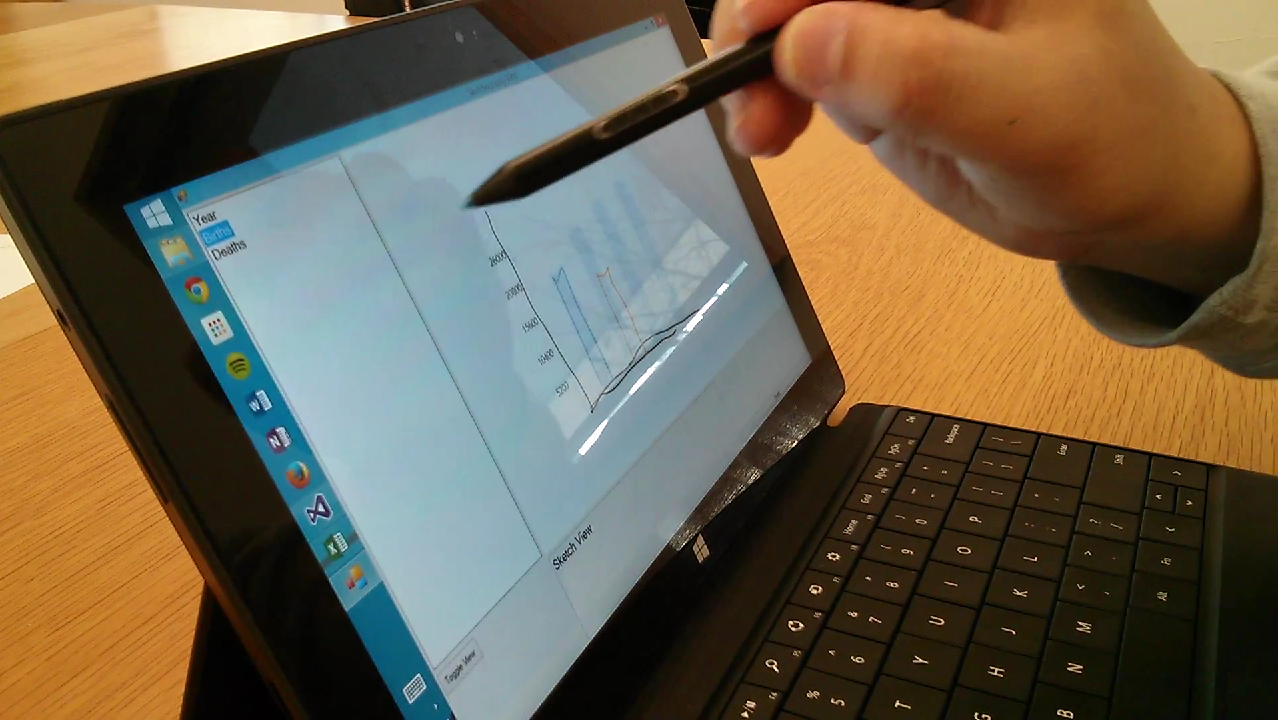
\includegraphics[width=0.7\linewidth]{PilotStudy1}
\caption{Screengrab from a video of the pilot study}
\end{figure}


The key things learnt were:
\begin{enumerate}
\item The task descriptions gave the steps in too much detail, as described above.
\item The width modification task was not appropriate, as described above.
\item Despite it being subtly mentioned that each chart element must be drawn with an individual stroke, some users draw both the X and Y axis in one stroke as an `L' shape. The program is modified before the final study to recognise these axes correctly and instantiate the two Axis objects accordingly. 
\end{enumerate}

There were no structural issues with the way the study itself was carried out, but the timing techniques and the script used during the demonstration did get refined with practice, making for a more valid final user study.

\section{User Study}
The final user study was conducted with the same structure as the pilot study since no issues were faced. To get a fair mix of native and non-native English speakers, it was carried out in Mumbai, India. 10 participants with various levels of experience with Excel, and aged between 20 and 60 years old, volunteered. They were all white collar workers in various industries, some of whom used computers on a daily basis.

\begin{table}
\begin{center}
\begin{tabular}{c c}
Age group & Number of participants \\
20-30 & 4 \\
30-40 & 1 \\
40-50 & 4 \\
50-60 & 1 \\

\end{tabular}
\end{center}
\caption{Distribution of participant ages}
\end{table}

One issue that the pilot study did not identify but was highlighted in the user study was the different ways people draw bars. Some of the Indian participants drew bars as two strokes, which none of the English participants had done. Thus, one of the strokes making up the bar would get recognised as an axis rather than a bar. This led to some interesting observations. The program has the ability to erase and redraw strokes that have been misclassified. However, for the purposes of the study, this feature was not demonstrated to users for 2 reasons:
\begin{enumerate}
\item The eraser is one of the less discoverable aspects of the application. Any of the participants could have noticed the eraser like shape at the end of the stylus and tried pressing it. I wanted to see if any users would discover this on their own, without being shown. None of the 10 did so, presumably because users have previously been familiar only with capacitative styluses that don't have such a feature. 
\item No matter how robust the stroke recogniser is made, there will be classification errors during usage. It was important to note how users react to this, understand what has happened, and correct the problem.
\end{enumerate} 

In practice, each of the users who made these split bars found a way around this. One took the less desirable option of hitting `Reset' and starting over, but the majority just drew over their previous sketches. When a new axis was drawn, the old, misinterpreted one was forgotten, and the chart got corrected. Then, the user would draw the bar with one stroke as required.

\subsection{Learnability}
Our hypothesis was that the time taken for the creation task the second time around would be lower, and this was confirmed by a Paired T Test as shown below.

%TODO Either change all commands to colour or change this back to black.
\begin{alltt}
> \hlkwd{t.test}\hlstd{(Task1, Task2,} \hlkwc{paired} \hlstd{=} \hlnum{TRUE}\hlstd{)}
\end{alltt}
\begin{verbatim} 
	Paired t-test

data:  Task1 and Task2
t = 5.2186, df = 9, p-value = 0.0005502
alternative hypothesis: true difference in means 
is not equal to 0
95 percent confidence interval:
 23.34058 59.05942
sample estimates:
mean of the differences 
                   41.2 
\end{verbatim}

%TODO Add boxplot and/or table showing mean/median differences.

The null hypothesis in the Paired T Test is that there is no difference in the Task 1 and Task 2 times for each participant. A $p-value < 0.05$ is considered to show that the two distributions are significantly different, and therefore the null hypothesis can be rejected. For every participant, there is a statistically significant difference in times between Task 1 and Task 2 - they were on average 41 seconds faster on their second try. The test is valid if the data follows a normal distribution, which a Q-Q plot and Shapiro-Wilk test suggested holds for this data.

\begin{table}[H]
\begin{center}
\setlength{\tabcolsep}{8pt} 
\renewcommand{\arraystretch}{1.5}


\begin{tabular}{l | l l}
Dataset & W & p-value \\ \hline
Task 1 & 0.8435 & 0.04854 \\
Task 2 & 0.8317 & 0.03511 \\
\end{tabular}
\end{center}
\caption{Creation task data was normally distributed}
\end{table}


\subsection{Modification}
The hypothesis was confirmed that people took significantly less time to modify the chart in Sketchography than they did in Excel.

A Paired T Test show this to be true ($p-value = 0.001389$), but was inconclusive since the data was not normal in this case ($p-value = 0.3966$ for Sketch and $0.1896$ for Excel). 

\begin{figure}[H]
		\centering
		\begin{subfigure}[b]{0.4\textwidth}
			\includegraphics[width=\textwidth]{figure/sketchqq.png}
		\end{subfigure}
		\begin{subfigure}[b]{0.4\textwidth}
			\includegraphics[width=\textwidth]{figure/excelqq.png}
		\end{subfigure}
		\caption{Modification task data wasn't normally distributed}
	\end{figure}

A Wilcox test, which doesn't rely on the same assumptions of normality, confirmed the hypothesis true. On average, each participant took 56 seconds fewer in Sketchography than in Excel.

\begin{verbatim}
	Wilcoxon rank sum test with continuity correction

data:  Sketch and Excel
W = 15.5, p-value = 0.01014
alternative hypothesis: true location shift is not equal to 0
\end{verbatim}

Qualitatively, a lot of participants were observed trying to drag the bounding box handles that appear when you select a bar in the Excel chart. They were frustrated when they realised that these handles can't actually be manipulated. One participant seemed to have prior experience with this - on reading the task, they said out loud, ``Oh yeah this is a pain, I know this is a pain".

Even when users did find relevant options in the Excel configuration panels, three of them hovered over the button, hesitated, and then tried something else instead. One actually said ``But this is different, no?", before abandoning it. They weren't able to instantly preview what result they would get if they picked the button, so they avoided exploring that possibility. 

On the other hand, they felt comfortable dragging the height handle in Sketchography despite it not having a label confirming its purpose.

One user even tried using the interface with a mouse, and by pinching her fingers apart on screen in a `zoom in' gesture. This suggests a willingness to experiment. It also suggested some future work for this project, to integrate finger gestures to manipulate the chart while using the pen purely for inking.

\subsection{Language Independence}
Half the participants spoke English as their primary language with native fluency, while the other half used it during their job but not as a primary language. Tests to show that the learnability for English speakers was more than that for non-English speakers failed. While not statistically conclusive, this suggests that there wasn't a significant difference in learnability depending on language, which supports the hypothesis.

\subsection{Other observations}
Given that some participants might have a lot of experience with Excel and none with Sketchography, making it an uneven playing field, data was collected about how frequently they use Excel. As might be expected, the less frequently the participant used Excel, in general, the bigger the gain in speed they got from using Sketchography for the Modification task. There aren't enough samples per frequency category (Daily, Weekly, \ldots) to run a conclusive statistical analysis, but the trend is visible in \autoref{fig:frequencybox}.

\begin{figure}[H]
\begin{center}
\includegraphics[width=0.8\linewidth]{figure/frequencybox.png}
\end{center}
\caption{Less frequent users of Excel gain a bigger speedup from using Sketchography}
\label{fig:frequencybox}
\end{figure}


No correlation was observed between the creation time task difference and the number of years the participant had used computers (Pearson's product-moment correlation $p-value = 0.1978$). Similarly, there was no correlation between creation time difference and the years of Excel use($p-value = 0.1386$).  

Interestingly, there is no correlation between the modification tasks time difference and whether the participant has used Excel for charting ($p-value = 0.5753$). This suggest that users might still not have learnt how to use Excel after having used it before, unlike Sketchography where they showed a measurable speedup after having used it once.

\subsection{Participant comments}
Some of the interesting responses to the open-ended questions are included below.

\textbf{Question: How do you think the software works?}

(Note: This question intended to elicit whether the participants had formed a correct mental model of how the software functions, but some of the participants less averse with English misinterpreted it as soliciting feedback, which led to even more interesting answers)

``Easy and real fast."

``Works pretty well. It is much easier to understand this software as compared to Excel."



\textbf{Question: What is the best thing about Excel?}

``Can easily plot the data and could be understood easily."

``All pervading."

\textbf{Question: What is the worst thing about Excel?}

``Certain times it is time consuming."

``Too vast to remember everything."

``Flexibility in charts is fairly low - it's templatized for the most part and not customize-able."

``Cumbersome."


\textbf{Question: What is the best thing about Sketchography?}

``Very efficient software. Easy to understand. Charts can be prepared in a matter of seconds."

``Intuitive."

\textbf{Question: What is the worst thing about Sketchography?}

``While making bars, not everybody will have the same style, so the Y Axis can get misjudged. Rest was easy and fun. Less time consuming. User friendly. Mistakes should get highlighted."

``The image recognition could be better. Apart from that, the software is easy to use, extremely intuitive, versatile and has great potential."

``A few kinks to work out, but on the right track."

\section{Summary}
In the introduction, this project outlined some hypotheses that it believed would be supported by the merits of the application. This chapter details a user study carried out on 10 participants that confirmed the two primary hypotheses with statistically significant results, and suggested that the third is supported too. Namely, users learn how to use the software on their first try and are already becoming skilled, and thus faster on their second try. They are also able to determine how to make a specific change quicker in Sketchography than they are in Microsoft Excel. It is likely that they have been able to learn how to use the application and make the modification regardless of how conversant they are in English.